\documentclass[fontset=windows]{article}
\usepackage{ctex}
\usepackage[margin=1in]{geometry}%设置边距,符合Word设定
\usepackage{listings}
\usepackage{color}
\usepackage[dvipsnames]{xcolor}
\usepackage{setspace}
\usepackage{booktabs,multirow}
\usepackage{float}
\usepackage{subfigure}
\usepackage[graphicx]{realboxes}
\usepackage[hidelinks]{hyperref}


\lstset{
    columns=fullflexible,
    language=bash,
    basicstyle=\ttfamily,
    showstringspaces=false,
    commentstyle=\color{BlueGreen},
    keywordstyle=\color{blue},
    breaklines=true, 
    frame=tb
}

\def\lstlistingname{代码}

\AtBeginDocument{\counterwithin{lstlisting}{section}}

\renewcommand\thefigure{\arabic{section}-\arabic{figure}}

\newcommand{\upcite}[1]{\textsuperscript{\cite{#1}}}

\title{\heiti\zihao{2} 操作系统课程设计实验报告}

\author{\fangsong 黄毅成}
\date{2024.7.16}

\begin{document}

\maketitle
\thispagestyle{empty}

\begin{center}
    \tableofcontents
\end{center}


\newpage

\section{Lab: Xv6 and Unix utilities}
\subsection{实验目的}

本实验旨在熟悉xv6操作系统及其系统调用。通过本次实验,我将学习如何在xv6环境中设置并运行操作系统,理解并实现基本的UNIX实用程序。这包括启动xv6、获取并管理源代码、编译和运行操作系统、以及实现和测试具体的系统调用和应用程序。本实验将帮助深入理解操作系统的运行机制和开发流程,为后续更复杂的操作系统编程打下坚实基础。

具体将实现以下程序:
\begin{itemize}
    \item sleep程序:编写一个xv6版本的sleep程序,使其根据用户指定的ticks暂停。
    \item pingpong程序:编写一个使用管道和fork系统调用在父子进程间传递字节的程序。
    \item primes程序:编写一个基于管道的并发素数筛选程序,将数值在进程间传递并筛选素数。
    \item find程序:编写一个简化版的find程序,遍历目录树查找特定文件名。
    \item xargs程序:编写一个简化版的xargs程序,从标准输入读取行并为每行运行一个命令。
\end{itemize}

在实现和测试这些系统调用的过程中,我们将深入理解操作系统的内部机制,并掌握如何在用户程序中调用这些功能。
\subsection{实验步骤}
\subsubsection{运行xv6}
\begin{enumerate}
    \item 利用以下指令获取Lab xv6源代码,查看util分支。
          \begin{lstlisting}
    $ git clone git://g.csail.mit.edu/xv6-labs-2021
    $ cd xv6-labs-2021
    $ git checkout util
        \end{lstlisting}
    \item 输入make qemu命令构建并运行xv6。
          \begin{lstlisting}
    $ make qemu
    
    ...

    xv6 kernel is booting

    hart 2 starting
    hart 1 starting
    init: starting sh
        \end{lstlisting}
\end{enumerate}

\subsubsection{实现sleep}

\begin{enumerate}
    \item 根据题目提示,可以实现如下代码:
          \begin{lstlisting}[language=c, title=sleep.c]
    #include "kernel/types.h"   // 包含内核类型定义
    #include "user/user.h"      // 包含用户模式下的库函数

    int main(int argc, char *argv[])
    {
        // 检查命令行参数是否等于2,即程序名和等待时间参数
        if (argc != 2)
        {
            fprintf(2, "Error: Parameters Error\n"); // 打印错误信息
            exit(1); // 退出程序,返回状态码1
        }

        sleep(atoi(argv[1])); // 调用 sleep 函数,等待指定的秒数

        exit(0); // 程序正常退出,返回状态码0
    }
        \end{lstlisting}
    \item 在 Makefile 文件中的UPROGS加上\$U/\_sleep\textbackslash 后利用make qemu命令编译启动xv6操作系统;
    \item 在xv6命令行中运行sleep,程序将暂停执行一段指定的时间:
          \begin{lstlisting}
    $ sleep 10
        \end{lstlisting}
\end{enumerate}

\subsubsection{实现pingpong}

\begin{enumerate}
    \item 首先创建两条管道和用于储存数据的缓冲区。
          \begin{lstlisting}[language=c,title=初始化管道和缓冲区]
    int fd1[2];
    int fd2[2];

    pipe(fd1);
    pipe(fd2);

    char buffer[16];
            \end{lstlisting}
    \item 利用fork()创建子进程。
          \begin{lstlisting}[language=c,title=fork()函数]
    if (fork() != 0)
    {
        // 父线程执行的代码...
    }
    else
    {
        // 子线程执行的代码...
    }
            \end{lstlisting}
    \item 在父进程中发送“ping”并接收“pong”。
          \begin{lstlisting}[language=c, title=父进程]
    // 父线程执行的代码
    write(fd1[1], "ping", strlen("ping"));
    read(fd2[0], buffer, 4);
    printf("%d: received %s\n", getpid(), buffer);
    \end{lstlisting}
    \item 在子进程中发送“pong”并接收“ping”。
          \begin{lstlisting}[language=c, title=子进程]
    // 子线程执行的代码
    read(fd1[0], buffer, 4);
    printf("%d: received %s\n", getpid(), buffer);
    write(fd2[1], "pong", strlen("pong"));
    \end{lstlisting}
    \item 把程序写在pingpong.c中,用同样的方法在xv6中运行程序,可以观察到父子进程分别输出的结果。
          \begin{lstlisting}
    $ pingpong
    5: received ping
    4: received pong
    \end{lstlisting}
\end{enumerate}

\subsubsection{实现 prime}
\begin{enumerate}
    \begin{figure}[h]
        \centering
        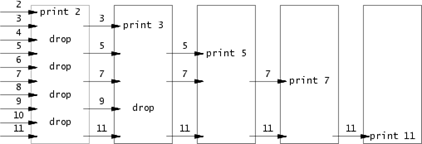
\includegraphics[width=\linewidth]{pics/图片1.png}
        \caption{primes程序原理}
        \label{fig:primes}
    \end{figure}
    \item 首先了解程序的原理。原理示意见图\ref{fig:primes}。程序通过递归创建进程和使用管道通信的方式,逐步筛选出素数。每个进程从管道中读取数值,将第一个数识别为素数,并过滤掉其倍数,然后将剩余的数传递给下一个进程继续处理,从而并发地筛选出所有素数。
    \item 把输出质数,创建子进程并向其传送数据的过程整合为一个递归函数。要注意文件描述符的回收,防止资源超限。
          \begin{lstlisting}[language=c, title=new\_prime\_proc函数的实现]
    void new_prime_proc(int *old_pipe)
    {
        close(old_pipe[1]); // 关闭旧管道的写端

        int first_num;
        // 从旧管道中读取第一个数,如果读取失败则退出
        if (!read(old_pipe[0], &first_num, sizeof(first_num)))
        {
            close(old_pipe[0]); // 关闭旧管道的读端
            exit(0);            // 退出进程
        }

        fprintf(1, "prime %d\n", first_num); // 打印第一个数,即当前的素数

        int new_pipe[2];
        pipe(new_pipe); // 创建新管道

        int p_id = fork(); // 创建子进程
        if (p_id == 0)
            new_prime_proc(new_pipe); // 子进程递归调用处理新管道
        else
        {
            int t;
            // 在父进程中,从旧管道中读取数,如果不是first_num的倍数则写入新管道
            while (read(old_pipe[0], &t, sizeof(t)))
            {
                if (t % first_num != 0)
                {
                    write(new_pipe[1], &t, sizeof(t));
                }
            }

            close(old_pipe[0]); // 关闭旧管道的读端
            close(new_pipe[0]); // 关闭新管道的读端
            close(new_pipe[1]); // 关闭新管道的写端

            wait((int *)0); // 等待子进程结束
        }
    }
    \end{lstlisting}
    \item 在主函数中将2~35写入管道,调用递归函数。
          \begin{lstlisting}[language=c, title=main()函数的实现]
    int main()
    {
        int p[2];
        pipe(p); // 创建管道
        int i;
        // 向管道中写入从2到35的所有数
        for (i = 2; i <= 35; i++)
            write(p[1], &i, sizeof(i));
        new_prime_proc(p); // 调用处理函数处理管道中的数
    
        exit(0); // 退出程序
    }
    \end{lstlisting}
    \item 把程序写在primes.c中,运行程序得到结果。
          \begin{lstlisting}
    $ primes
    prime 2
    prime 3
    ...
    prime 31
    \end{lstlisting}
\end{enumerate}

\subsubsection{实现 find}

\begin{enumerate}
    \item 首先,仿照ls.c实现一个辅助函数char*fmtname(char *path),把路径末尾的文件名提取出来,实现过程略。
    \item 利用深度优先搜索的思想,实现一个find函数递归寻找文件。
          \begin{lstlisting}[language=c, title=find函数的实现]
    void find(char *path, char *target)
    {
        char buf[512], *p;
        int fd;
        struct dirent de;
        struct stat st;

        // 打开指定路径的文件或目录
        if ((fd = open(path, 0)) < 0)
        {
            fprintf(2, "find: cannot open %s\n", path);
            return;
        }

        // 获取文件或目录的状态信息
        if (fstat(fd, &st) < 0)
        {
            fprintf(2, "find1: cannot stat %s\n", path); 
            close(fd);
            return;
        }

        // 根据文件或目录的类型进行处理
        switch (st.type)
        {
        case T_FILE:
            // 如果是文件,比较文件名是否与目标名称相同
            if (strcmp(target, path2name(path)) == 0)
            {
                printf("%s\n", path); // 输出文件路径
            }

            break;
        case T_DIR:
            // 如果是目录,检查路径长度是否超出缓冲区范围
            if (strlen(path) + 1 + DIRSIZ + 1 > sizeof buf)
            {
                printf("find: path too long\n"); // 输出错误信息,路径过长
                break;
            }
            strcpy(buf, path); // 将路径复制到缓冲区
            p = buf + strlen(buf);
            *p++ = '/';

            // 遍历目录中的每个文件或子目录
            while (read(fd, &de, sizeof(de)) == sizeof(de))
            {
                if (de.inum == 0)
                    continue; // 跳过空目录项

                memmove(p, de.name, DIRSIZ); // 将文件或目录名复制到缓冲区末尾
                p[DIRSIZ] = 0;               // 添加字符串结束符

                // 获取文件或目录的状态信息
                if (stat(buf, &st) < 0)
                {
                    // 输出错误信息,无法获取文件或目录的状态信息
                    printf("find2: cannot stat %s\n", buf); 
                    continue;
                }

                // 排除当前目录和上级目录的特殊情况
                if (strlen(de.name) == 1 && de.name[0] == '.')
                    continue;
                if (strlen(de.name) == 2 
                && de.name[0] == '.' 
                && de.name[1] == '.')
                    continue;
                find(buf, target); // 递归调用查找函数,继续查找子目录
            }
            break;
        }

        close(fd); // 关闭文件或目录
    }
    \end{lstlisting}
    \item 在主函数中调用find函数。
    \item 将程序写在find.c中,运行程序得到结果。
          \begin{lstlisting}
    $ find . b
    ./a/b
    ./b
    \end{lstlisting}
\end{enumerate}

\subsubsection{实现 xargs}
\begin{enumerate}
    \item 首先初始化一些变量。
          \begin{lstlisting}[language=c, title=初始化]
    int i;
    int arg_count = 0;  // 参数数量计数器
    char *args[MAXARG]; // 参数数组,最大长度为MAXARG
    int initial_arg_count = arg_count; // 存储初始参数数量的位置
    
    int line_index = 0; // 当前行的索引
    char input_char;                   // 用于读取字符
    char *current_line;                // 指向当前处理的行
    char line_buffer[512];             // 临时存储字符串的缓冲区
    current_line = line_buffer;

    // 将命令行参数复制到参数数组args中
    for (i = 1; i < argc; ++i)
    {
        args[arg_count++] = argv[i];
    }
    \end{lstlisting}
    \item 循环处理读取的字符。
          \begin{lstlisting}[language=c, title=输入处理循环]
    while (read(0, &input_char, 1) > 0)
    {
        // 对输入字符的操作...
    }
    \end{lstlisting}
    \item 循环中的字符处理:\begin{itemize}
              \item 对于普通字符,将其加入到当前行末尾;
              \item 遇到空格,表示一个参数已经结束,将参数添加到参数列表之中;
                    \begin{lstlisting}[language=c, title=空格的处理]
    current_line[line_index] = '\0';  // 添加字符串结束符
    line_index = 0;                   // 重置索引
    args[arg_count++] = current_line; // 将当前单词添加到参数数组
    char line_buffer[512];            // 重新分配缓冲区
    current_line = line_buffer;
        \end{lstlisting}
              \item 遇到回车,表示一行结束,将最后一个参数加入参数列表之中并执行命令。
                    \begin{lstlisting}[language=c, title=回车的处理]
    // 处理换行符,将当前行作为参数
    current_line[line_index] = '\0'; // 添加字符串结束符
    line_index = 0;                  // 重置索引

    args[arg_count++] = current_line; // 将当前行添加到参数数组
    args[arg_count] = 0;              // 设置参数数组的结束标志

    if (fork()) // 创建子进程
    {
        wait(0);                       // 父进程等待子进程结束
        arg_count = initial_arg_count; // 重置参数数量
    }
    else
    {
        exec(argv[1], args); // 子进程执行命令
    }
            \end{lstlisting}
          \end{itemize}
    \item 将程序写入xargs.c中,运行程序得到结果。
          \begin{lstlisting}
    $ echo hello too | xargs echo bye 
    bye hello too
    \end{lstlisting}
\end{enumerate}

\subsection{评测结果}

利用./grade-lab-util脚本评测,得到结果见图\ref{fig:util}
\begin{figure}[h]
    \centering
    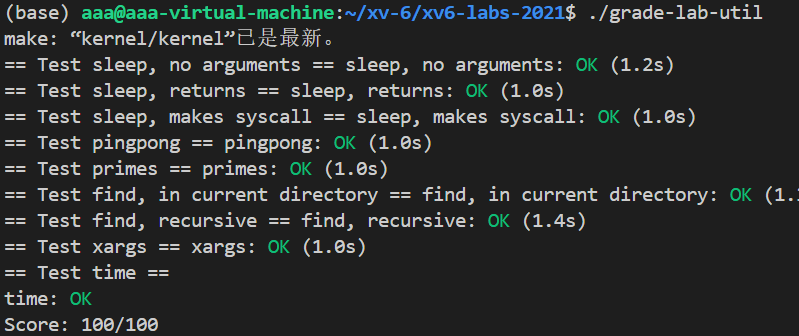
\includegraphics[width=\linewidth]{pics/util评测结果.png}
    \caption{评测结果}
    \label{fig:util}
\end{figure}

\subsection{实验小结}
本实验中我初步了解了xv6这个操作系统的基本结构。了解了其利用qemu模拟器运行、编程的基本方法。本实验中需要实现的多为基本的系统功能,让我对Unix操作系统有了更深入的了解。

此外primes是我认为这里面最难的程序。首先,理解这个程序的实现原理就花费了我不少时间。在之后实现这个程序的过程之中,我在处理管道、父子进程的关系的时候遇到了一些困难。不过最后我还是成功实现了程序,这对我理解管道、进程并行有很大的帮助。

\section{Lab: System calls}

\subsection{实验目的}

本实验旨在进一步熟悉系统调用,重点掌握如何添加系统调用,理解系统调用的工作原理,内核态和用户态的联系。

本实验实现了两个系统调用:
\begin{itemize}
    \item System call tracing:实现对系统调用的跟踪;
    \item Sysinfo:收集有关正在运行的系统的信息。
\end{itemize}

\subsection{实验步骤}

\subsubsection{实现trace}

\begin{enumerate}
    \item 首先,根据提示,在Makefile的UPROGS中添加\$U/\_trace\textbackslash。
    \item 在user.h文件的system calls部分添加trace函数。
          \newpage
          \begin{lstlisting}[language=c, title=对user.h的改动]
    // system calls
    int fork(void);
    ...
    // 添加 trace函数
    int trace(int);
    \end{lstlisting}
    \item 在usys.pl末尾添加entry("trace");以便在汇编语言中添加这个函数。
    \item 进入kernel文件夹,在syscall.h中添加SYS\_trace系统调用号的定义,值往下类推,即为22。
          \begin{lstlisting}[language=c, title=对syscall.h的更改]
    // System call numbers
    #define SYS_fork 1
    ...
    // 为trace添加系统调用号
    #define SYS_trace 22
          \end{lstlisting}
    \item 更改进程结构体。在proc.h中的进程结构体最后添加一个掩码trace\_mask,用于记录哪些进程要被追踪。
          \begin{lstlisting}[language=c, title=对进程结构体的更改]
    struct proc
    {
        struct spinlock lock;
        ...
        // 添加掩码
        int trace_mask;
    };
    \end{lstlisting}
    \item 在sysproc.c文件中,添加系统调用函数sys\_trace,在调用时设置掩码。
          \begin{lstlisting}[language=c, title=实现sys\_trace系统调用]
    uint64 sys_trace(void)
    {
        // 获取参数
        int mask;
        if (argint(0, &mask) < 0)
            return -1;
        // 获取当前进程
        struct proc *p = myproc();
        // 写入掩码
        p->trace_mask = mask;
        return 0;
    }
    \end{lstlisting}
    \item 在syscall.c中修改syscall函数,使其根据掩码判断是否输出当前调用信息。
          \begin{lstlisting}[language=c, title=对syscall函数的修改]
    void syscall(void)
    {
        int num;
        struct proc *p = myproc();

        num = p->trapframe->a7;
        if (num > 0 && num < NELEM(syscalls) && syscalls[num])
        {
            p->trapframe->a0 = syscalls[num]();

            // 获得掩码
            int trace_mask = p->trace_mask;

            // 如果掩码对应,输出当前系统调用信息
            if ((trace_mask >> num) & 1)
            {
                printf("%d: syscall %s -> %d\n", 
                        p->pid, 
                        syscall_names[num - 1], 
                        p->trapframe->a0);
            }
        }
        else
        {
            ...
        }
    }
    \end{lstlisting}
    \item 修改proc.c中的freeproc函数和fork函数,确保掩码在进程释放时重置掩码、在子进程创建时传递掩码。
          \newpage
          \begin{lstlisting}[language=c, title=对proc.c的修改]
    static void freeproc(struct proc *p)
    {
        if (p->trapframe)
        kfree((void *)p->trapframe);
        ...

        // 添加了这一行
        p->trace_mask = 0;
    }

    int fork(void)
    {
        ...

        // 把子进程的掩码也设置为与父进程相同
        np->trace_mask = p->trace_mask;

        ...
    }
    \end{lstlisting}
\end{enumerate}

\subsubsection{实现sysinfo}
\begin{enumerate}
    \item 首先,先仿照trace中的方法,在Makefile、syscall.h、syscall.c、user.h、user.pl中注册名为sysinfo的系统调用。
    \item 在kalloc.c中仿照kalloc函数读取空闲内存链表的方式,实现一个计算空闲内存空间大小的函数acquire\_freeman。
          \begin{lstlisting}[language=c, title=acquire\_freemem的实现]
    uint64 acquire_freemem()
    {
        struct run *r;
        uint64 cnt = 0;

        // 锁
        acquire(&kmem.lock);
        r = kmem.freelist;
        // 遍历链表
        while (r)
        {
            r = r->next;
            cnt++;
        }
        // 释放锁
        release(&kmem.lock);
        // 返回空间大小(页数乘页尺寸)
        return cnt * PGSIZE;
    }
    \end{lstlisting}
    \item 在proc.c中,实现一个计算非使用状态进程个数的函数acquire\_nproc,利用记录进程的数组struct proc proc[NPROC]。
          \begin{lstlisting}[language=c, title=acquire\_nproc的实现]
    uint64 acquire_nproc()
    {
        struct proc *p;
        int cnt = 0;
    
        for (p = proc; p < &proc[NPROC]; ++p)
        {
            acquire(&p->lock);
            if (p->state != UNUSED)
                cnt++;
            release(&p->lock);
        }
    
        return cnt;
    }    
    \end{lstlisting}
    \item 最后,在sysproc.c中完成sys\_sysinfo函数的实现。利用argaddr读取参数的地址,利用copyout对地址进行写入。
          \begin{lstlisting}[language=c, title=sys\_sysinfo的实现]
    uint64 sys_sysinfo(void)
    {
        struct sysinfo info;
        uint64 addr;
        struct proc *p = myproc();

        // 计算空闲进程数
        info.nproc = acquire_nproc();
        // 计算空闲内存数
        info.freemem = acquire_freemem();

        // 获取参数
        if (argaddr(0, &addr) < 0)
            return -1;
        // 写入结构体
        if (copyout(p->pagetable, addr, (char *)&info, sizeof(info)) < 0)
            return -1;
        return 0;
    }
    \end{lstlisting}
\end{enumerate}

\subsection{评测结果}
利用grade-lab-syscall脚本评测,得到评测结果如图\ref{fig:syscall}所示。
\begin{figure}[h]
    \centering
    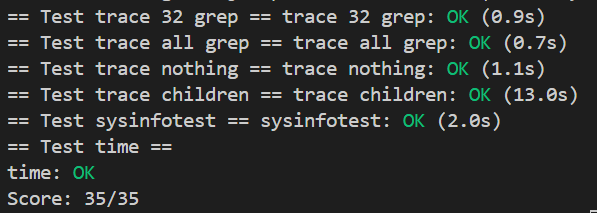
\includegraphics[width=\linewidth]{pics/syscall评测结果.png}
    \caption{评测结果}
    \label{fig:syscall}
\end{figure}

\subsection{实验小结}

在本实验中,我实现了两个系统调用。通过实验,我了解到了在内核中实现系统调用的一整套流程。

在实验中,为了实现我自己的系统调用,我阅读了许多kernel的代码,对内核有了更好的了解。通过仿照内核代码中一些函数的实现以及提示,我才得以完成我自己的系统调用。我在阅读内核代码的时候也遇到了一些困难,花费了不少时间来理解代码的含义。

这次实验大大加深了我对系统调用的了解,为之后的实验打下基础。


\section{Lab: Page tables}
\subsection{实验目的}

本实验中将涉及到操作系统中重要的\textbf{页表}概念。操作系统中的页表是一种数据结构,用于实现虚拟内存和物理内存之间的地址映射。每个进程都有自己的页表,将虚拟地址映射到物理地址,从而使得操作系统能够有效地管理内存,提供内存保护和共享内存功能。页表的概念对于操作系统课程至关重要,因为它涉及到内存管理、进程隔离和系统性能等核心问题。理解页表如何工作,有助于深入掌握操作系统的内存管理机制,了解虚拟内存的实现细节,并且能够解决与内存管理相关的各种问题。

本实验中将探索页表的具体操作并对其进行修改,以加快某些系统调用并检测哪些页面被访问。具体将实现以下内容:
\begin{itemize}
    \item 利用页表加速系统调用;
    \item 打印页表;
    \item 检测被访问的页表。
\end{itemize}

\subsection{实验步骤}

\subsubsection{实现系统调用加速}
\begin{enumerate}
    \item 首先,在proc.c文件中修改proc\_pagetable函数,仿照前面的代码添加用户页表的映射,注意内存权限应为PTE\_U。
          \begin{lstlisting}[language=c, title=对proc\_pagetable函数的修改]
    pagetable_t proc_pagetable(struct proc *p)
    {
        pagetable_t pagetable;

        ...

        // 添加的部分
        if (mappages(pagetable, USYSCALL, PGSIZE,
                    (uint64)(p->usyscall), PTE_R | PTE_U) < 0)
        {
            uvmunmap(pagetable, USYSCALL, 1, 0);
            uvmunmap(pagetable, TRAMPOLINE, 1, 0);
            uvmfree(pagetable, 0);
            return 0;
        }

        return pagetable;
    }
    \end{lstlisting}
    \item 在proc.c文件中修改allocproc函数,仿照前面的代码,给进程分配用户页表。
          \begin{lstlisting}[language=c, title=对allocproc函数的修改]
    static struct proc * allocproc(void)
    {
        ...
    
        // 添加的部分
        if ((p->usyscall = (struct usyscall *)kalloc()) == 0)
        {
            freeproc(p);
            release(&p->lock);
            return 0;
        }
        p->usyscall->pid = p->pid;
    
        ...

        return p;
    }
    \end{lstlisting}
    \item 在proc.c文件中修改freeproc函数,仿照前面的代码,释放用户页表。
          \begin{lstlisting}[language=c, title=对freeproc函数的修改]
    freeproc(struct proc *p)
    {
        ...
        // 添加的部分
        if (p->usyscall)
        kfree((void *)p->usyscall);
        p->usyscall = 0;
        ...
    }
    \end{lstlisting}
    \item 如此设置,系统就能利用用户页表实现更快地进程号查询,从而加速系统调用。
\end{enumerate}

\subsubsection{实现页表打印}
\begin{enumerate}
    \item 首先,阅读vm.c文件中freewalk函数的代码,了解如何对页表项进行递归遍历和访问。
          \begin{lstlisting}[language=c, title=freewalk函数的原型]
    // Recursively free page-table pages.
    // All leaf mappings must already have been removed.
    void freewalk(pagetable_t pagetable)
    {
        // there are 2^9 = 512 PTEs in a page table.
        for (int i = 0; i < 512; i++)
        {
            pte_t pte = pagetable[i];
            if ((pte & PTE_V) && (pte & (PTE_R | PTE_W | PTE_X)) == 0)
            {
                // this PTE points to a lower-level page table.
                uint64 child = PTE2PA(pte);
                freewalk((pagetable_t)child);
                pagetable[i] = 0;
            }
            else if (pte & PTE_V)
            {
                panic("freewalk: leaf");
            }
        }
        kfree((void *)pagetable);
    }
    \end{lstlisting}
    \item 仿照freewalk函数,实现递归打印页表的vmprint函数
          \begin{lstlisting}[language=c, title=vmprint函数的实现]
    void vmprint(pagetable_t pagetable, uint64 depth)
    {
        // 如果递归深度大于2,则直接返回,RISC-V只有三级页表
        if (depth > 2)
        return;
    
        // 如果是最顶层页表,打印页表的地址
        if (depth == 0)
        {
            printf("page table %p\n", pagetable);
        }
    
        // 定义一个静态的前缀数组,用于打印格式化输出
        static char *prefix[] = {"..", ".. ..", ".. .. .."};
    
        // 页表中有2^9 = 512个页表项
        for (int i = 0; i < 512; i++)
        {
            pte_t pte = pagetable[i];  // 获取当前页表项
            if (pte & PTE_V)  // 如果页表项有效
            {
                // 打印当前页表项的信息,包括前缀、索引、页表项和物理地址
                printf("%s%d: pte %p pa %p\n", prefix[depth], i, pte, PTE2PA(pte));
                uint64 child = PTE2PA(pte);  // 获取下一级页表的物理地址
                vmprint((pagetable_t)child, depth + 1);  // 递归打印下一级页表
            }
        }
    }
    \end{lstlisting}
    \item 在def.h中声明vmprint函数以便调用。
    \item 在exec.c文件中,对exec函数进行修改,调用vmprint函数,使其在进程号为1是打印页表。
          \begin{lstlisting}[language=c, title=对exec函数的修改]
    int exec(char *path, char **argv)
    {
        ...
        
        // 添加的语句
        if (p->pid == 1)
            vmprint(p->pagetable, 0);

        ...
    }    
    \end{lstlisting}
\end{enumerate}
\subsubsection{实现被访问页面侦测}
\begin{enumerate}
    \item 首先,在riscv.h文件中添加一个PTE\_A常量,查阅RISC-V手册可知其值应为0b00100000,即$2^6$。
          \begin{lstlisting}[language=c, title=PTE\_A的定义]
    #define PTE_A (1L << 6)    
    \end{lstlisting}
    \item 在vm.c文件中实现vm\_pgaccess函数,利用PTE\_A标志判断给定虚拟地址的页表项是否被访问,若被访问返回1并清除PTE\_A标志。在def.h中添加函数的声明。
          \begin{lstlisting}[language=c, title=vm\_pgaccess函数的实现]
    int vm_pgaccess(pagetable_t pagetable, uint64 va)
    {
        pte_t *pte;  // 页表项指针
    
        // 如果虚拟地址超出最大允许值,返回0
        if (va >= MAXVA)
            return 0;
    
        // 获取虚拟地址对应的页表项指针
        pte = walk(pagetable, va, 0);
        // 如果页表项不存在,返回0
        if (pte == 0)
            return 0;
    
        // 如果页表项的访问标志位被设置
        if ((*pte & PTE_A) != 0)
        {
            // 清除访问标志位
            *pte = *pte & (~PTE_A);
            // 返回1表示访问标志位被清除
            return 1;
        }
    
        // 如果访问标志位未设置,返回0
        return 0;
    }
    \end{lstlisting}
    \item 在sysproc.c中补全sys\_pgaccess系统调用,使之能够把页面访问的情况记录在掩码之中。
          \begin{lstlisting}[language=c, title=sys\_pgaccess函数的实现]
    int sys_pgaccess(void)
    {
        uint64 addr;  // 内存起始地址
        int len;      // 内存区域的页数
        int bitmask;  // 存储结果的用户地址
    
        // 获取系统调用的第一个参数(内存起始地址),并检查是否成功
        if (argaddr(0, &addr) < 0)
            return -1;
    
        // 获取系统调用的第二个参数(内存区域的页数),并检查是否成功
        if (argint(1, &len) < 0)
            return -1;
    
        // 获取系统调用的第三个参数(存储结果的用户地址),并检查是否成功
        if (argint(2, &bitmask) < 0)
            return -1;
    
        // 检查页数是否在合理范围内(0到32页)
        if (len > 32 || len < 0)
            return -1;
    
        int res = 0;  // 用于存储访问标志结果
        int i;
        struct proc *p = myproc();  // 获取当前进程结构体
    
        // 遍历每一页,检查访问标志并存储结果
        for (i = 0; i < len; i++)
        {
            int va = addr + i * PGSIZE;  // 计算每一页的虚拟地址
            int abit = vm_pgaccess(p->pagetable, va);  // 检查页表项的访问标志
        
            res = res | abit << i;  // 将访问标志结果合并到res中
        }
    
        // 将结果拷贝到用户空间,如果失败则返回-1
        if (copyout(p->pagetable, bitmask, (char *)&res, sizeof(res)) < 0)
            return -1;
    
        // 成功返回0
        return 0;
    }      
    \end{lstlisting}
\end{enumerate}

\subsection{评测结果}
利用 grade-lab-pgtbl 脚本评测,得到评测结果如图\ref{fig:pgtbl}所示。
\begin{figure}[h]
    \centering
    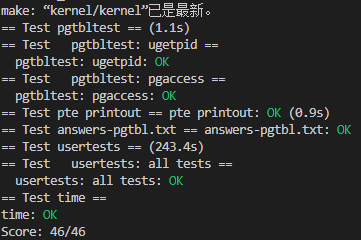
\includegraphics[width=\linewidth]{pics/pagetable评测结果.png}
    \caption{评测结果}
    \label{fig:pgtbl}
\end{figure}

\subsection{实验小结}
在本次实验中,我深入探索了操作系统中的页表概念,并通过一系列具体的实现来加深对该概念的理解。页表是操作系统中管理虚拟内存的重要数据结构,它通过将虚拟地址映射到物理地址,实现内存保护和内存共享功能。我通过本实验的操作,掌握了页表的操作方法和实现细节。

我在本实验上花费了不少时间,复习了操作系统课上讲过的页表概念,并研究内核代码。实验总体来说是有些难度。

在实验过程中,我不仅巩固了操作系统中页表的基本概念,还通过实际编程和调试,掌握了页表的具体实现方法和应用场景。通过这些实践操作,我更深入地理解了操作系统的内存管理机制,并积累了宝贵的编程经验和调试技巧。这些知识和技能对于我后续解决实际问题将大有裨益。


\end{document}
